%%%%%%%%%%%%%%%%%%%%%%%%%%%%%%%%%%%%%%%%%%%%%%%%%%%%%%%%
%%%%                                              %%%%%%
%%%%  Author: Peter Wilson                        %%%%%%
%%%%                                              %%%%%%
%%%%  ANDES quad element                          %%%%%%
%%%%                                              %%%%%%
%%%%%%%%%%%%%%%%%%%%%%%%%%%%%%%%%%%%%%%%%%%%%%%%%%%%%%%%


%fref generates automatically the respective abreviation/word in the text for the reference. You just have to define a label starting with the respective keyword.
%english: chap, sec, fig, eq, app
%deutsch: chap/kap, abs, abb, gl, anh
%see http://ctan.space-pro.be/tex-archive/macros/latex/contrib/fancyref/fancyref.pdf for more information

\renewcommand{\Thema}{Benchmarking}



\chapter{Benchmarking}

Benchmarking yeah

\section{Shell obstacle course}

To test the correct derivation and implementation of the thin quad shell element, the shell obstacle course proposed by Belytschko \cite{Bel85} is considered.

\subsection{Scordelis-Lo roof}

The Scordelis-Lo roof is part of a cylindrical shell fixed by rigid diaphragms at it's axial ends. The only loading is a pseudo-gravity distributed load that has a magnitude of 90. Due to symmetry only a quarter of the shell is modelled. The key result is the vertical displacement of the lateral side at the midpoint, denoted by $\textcolor{red}{u}$ in the following diagram. The reference value is $u_{ref} = 0.3024$.

\begin{figure}[H]
	\centering
	\def\svgwidth{\columnwidth}
	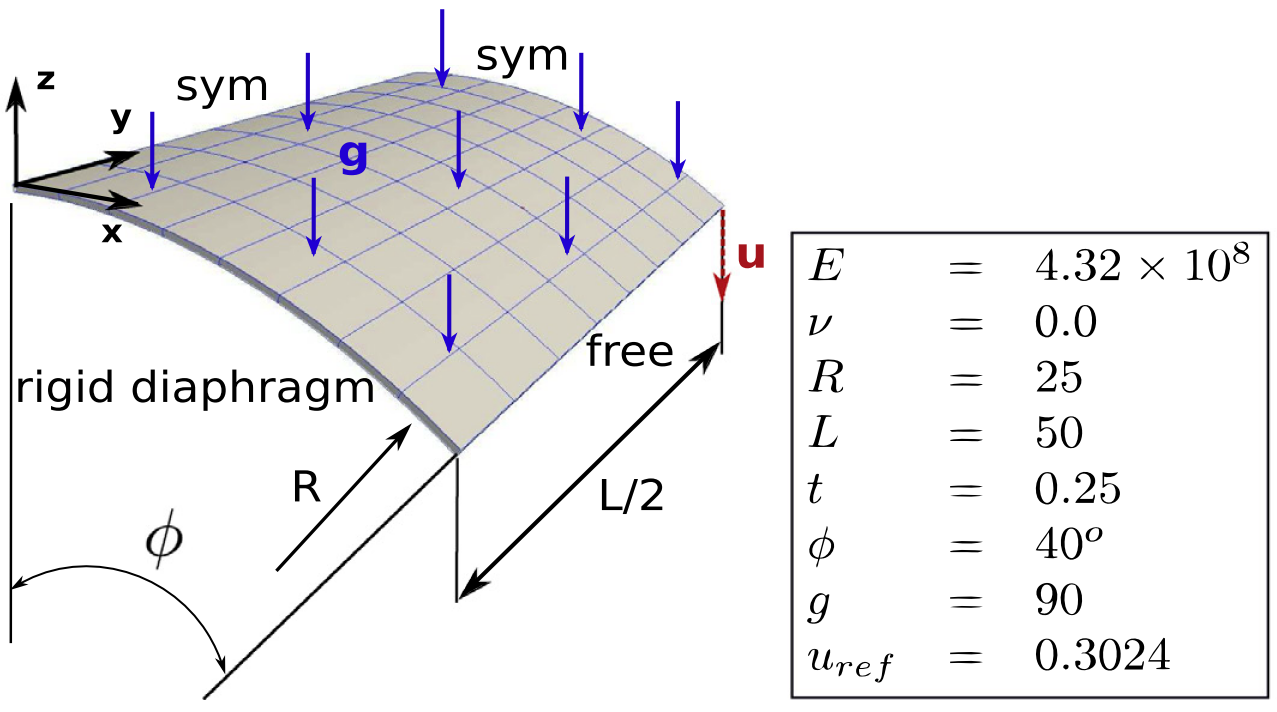
\includegraphics[width=8cm]{images/scordelisroof.png}
	\caption{Problem definition of the Scordelis-Lo roof benchmark (source: \cite{Bou13})}
	\label{scordelisroof}
\end{figure}

\pgfplotsset{width=6cm}
\begin{figure}[H]
	\centering
	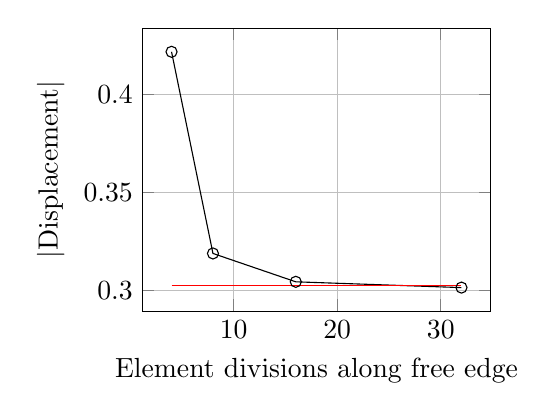
\begin{tikzpicture}
	\begin{axis}[
	xlabel=Element divisions along free edge,
	ylabel=$|$Displacement$|$,
	grid=both,]
	\addplot[color=black,mark=o] coordinates {
		(4,0.42177)
		(8,0.31887)
		(16,0.3044)
		(32,0.30145)};
	\addplot[red,domain=4:32] 
	{0.3024};
	\end{axis}
	\end{tikzpicture}
	\caption{Element convergence for the Scordelis-Lo roof benchmark}
	\label{scordelisroofbench}
\end{figure}



The performance of the element is demonstrated in the convergence graph above. It is clear that the element agrees with the reference solution.

\subsection{Pinched cylinder}

The pinched cylinder considers a cylindrical shell fixed by rigid diaphragms at it's axial ends. The loading consists of two opposing compressive point loads at the centre of the shell. Due to symmetry only an eighth of the shell is modelled. The key result is the vertical displacement under the point load, denoted by $\textcolor{red}{u}$ in the following diagram. The reference value is $u_{ref} =  1.8248\ \times\ 10^{-5}$. 

\begin{figure}[H]
	\centering
	\def\svgwidth{\columnwidth}
	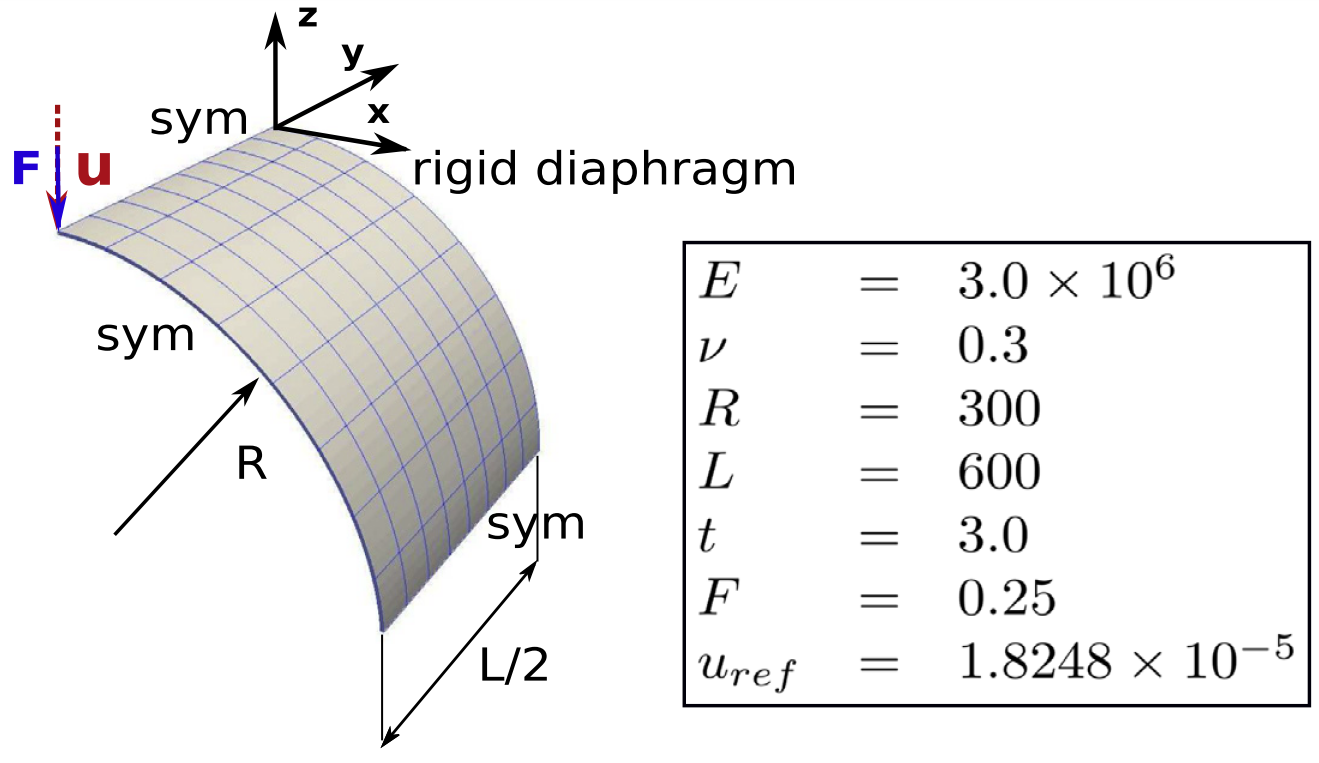
\includegraphics[width=8cm]{images/pinchedcylinder.png}
	\caption{Problem definition of the pinched cylinder benchmark (source: \cite{Bou13})}
	\label{pinchedcylinder}
\end{figure}


\pgfplotsset{width=6cm}
\begin{figure}[H]
	\centering
	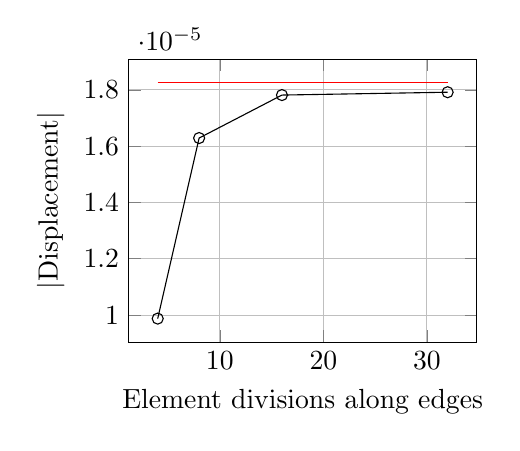
\begin{tikzpicture}
	\begin{axis}[
	xlabel=Element divisions along edges,
	ylabel=$|$Displacement$|$,
	grid=both,]
	\addplot[color=black,mark=o] coordinates {
		(4,0.0000098753)
		(8,0.0000162870)
		(16,0.0000178130)
		(32,0.0000179140)};
	\addplot[red,domain=4:32] 
	{0.000018248};
	\end{axis}
	\end{tikzpicture}
	\caption{Element convergence for the pinched cylinder benchmark}
	\label{pinchedcylinderbench}
\end{figure}



The performance of the element is demonstrated in the convergence graph above. It is clear that the element agrees with the reference solution.

\subsection{Pinched hemisphere}

The pinched hemisphere considers a hemispherical shell loaded with opposing point loads along it's equator. Due to symmetry only a quarter of the shell is modelled. The key result is the 'x' displacement along one of the point loads, denoted by $\textcolor{red}{u}$ in the following diagram. The reference value is $u_{ref} =  0.0924$. 

\begin{figure}[H]
	\centering
	\def\svgwidth{\columnwidth}
	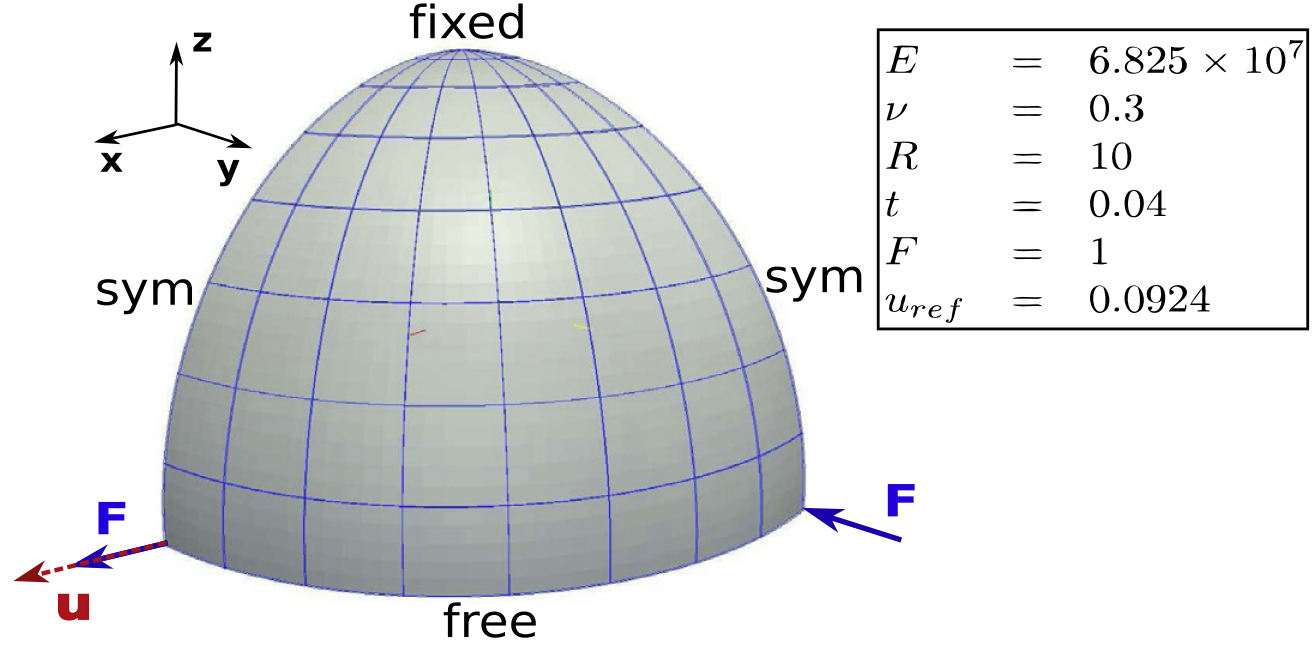
\includegraphics[width=8cm]{images/pinchedhemisphere.png}
	\caption{Problem definition of the pinched hemisphere benchmark (source: \cite{Bou13})}
	\label{pinchedhemisphere}
\end{figure}

\pgfplotsset{width=6cm}
\begin{figure}[H]
	\centering
	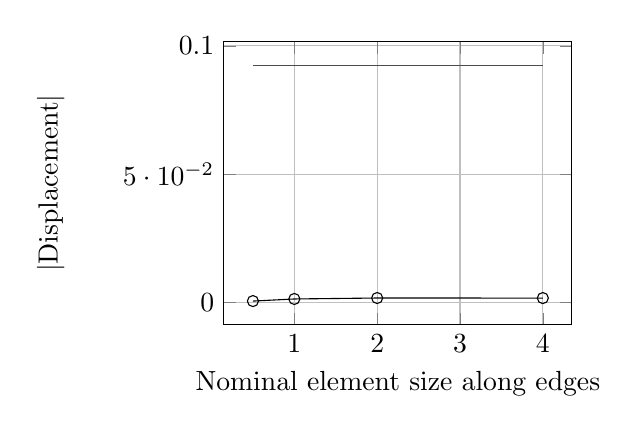
\begin{tikzpicture}
	\begin{axis}[
	xlabel=Nominal element size along edges,
	ylabel=$|$Displacement$|$,
	ylabel style={yshift=0.5cm},
	grid=both,]
	\addplot[color=black,mark=o] coordinates {
		(4,0.001648235)
		(2,0.001670075)
		(1,0.001297573)
		(0.5,0.000476183)};
	\addplot[red,domain=0.5:4] 
	{0.0924};
	\end{axis}
	\end{tikzpicture}
	\caption{Element convergence for the pinched hemisphere benchmark}
	\label{pinchedhemispherebench}
\end{figure}

Contrary to the previous benchmarks, the element does not converge to the reference solution in the pinched hemisphere test.  A key point to note is that the other benchmarks in the shell obstacle course employ a structured mesh, while the geometry of this test requires an unstructured mesh. Subsequent investigations of the element attempting to isolate remaining formulation issues have revealed the following phenomena:

\begin{itemize}
	\item Membrane tests
	\begin{itemize}
		\item[{$\times$}] Membrane tests with coarse structured meshes yield incorrect results
		\item[{$\checkmark$}] Membrane tests with fine structured meshes yield correct results
		\item[{$\times$}] Membrane tests with unstructured meshes ranging from coarse to fine yield incorrect results
	\end{itemize}
	
	\item Bending tests
	\begin{itemize}
		\item[{$\checkmark$}] Bending tests with structured meshes ranging from coarse to fine achieve correct results
		\item[{$\times$}] Bending tests with unstructured meshes ranging from coarse to fine yield incorrect results
	\end{itemize}	
\end{itemize}

From the above statements, it can be concluded that: (1) the performance of the membrane formulation is dependent on mesh refinement, and (2) the element currently handles unstructured meshes incorrectly.













\section{Geometically nonlinear benchmarks}

asdfasdf

\subsection{Hinged cylindrical roof}

Tests snapthrough

\singlespacing
\begin{figure}[H]
	%\centering
	\subfloat[Hinged cylindrical roof definition \cite{Sze2004}]
	{\label{ref_label1}
		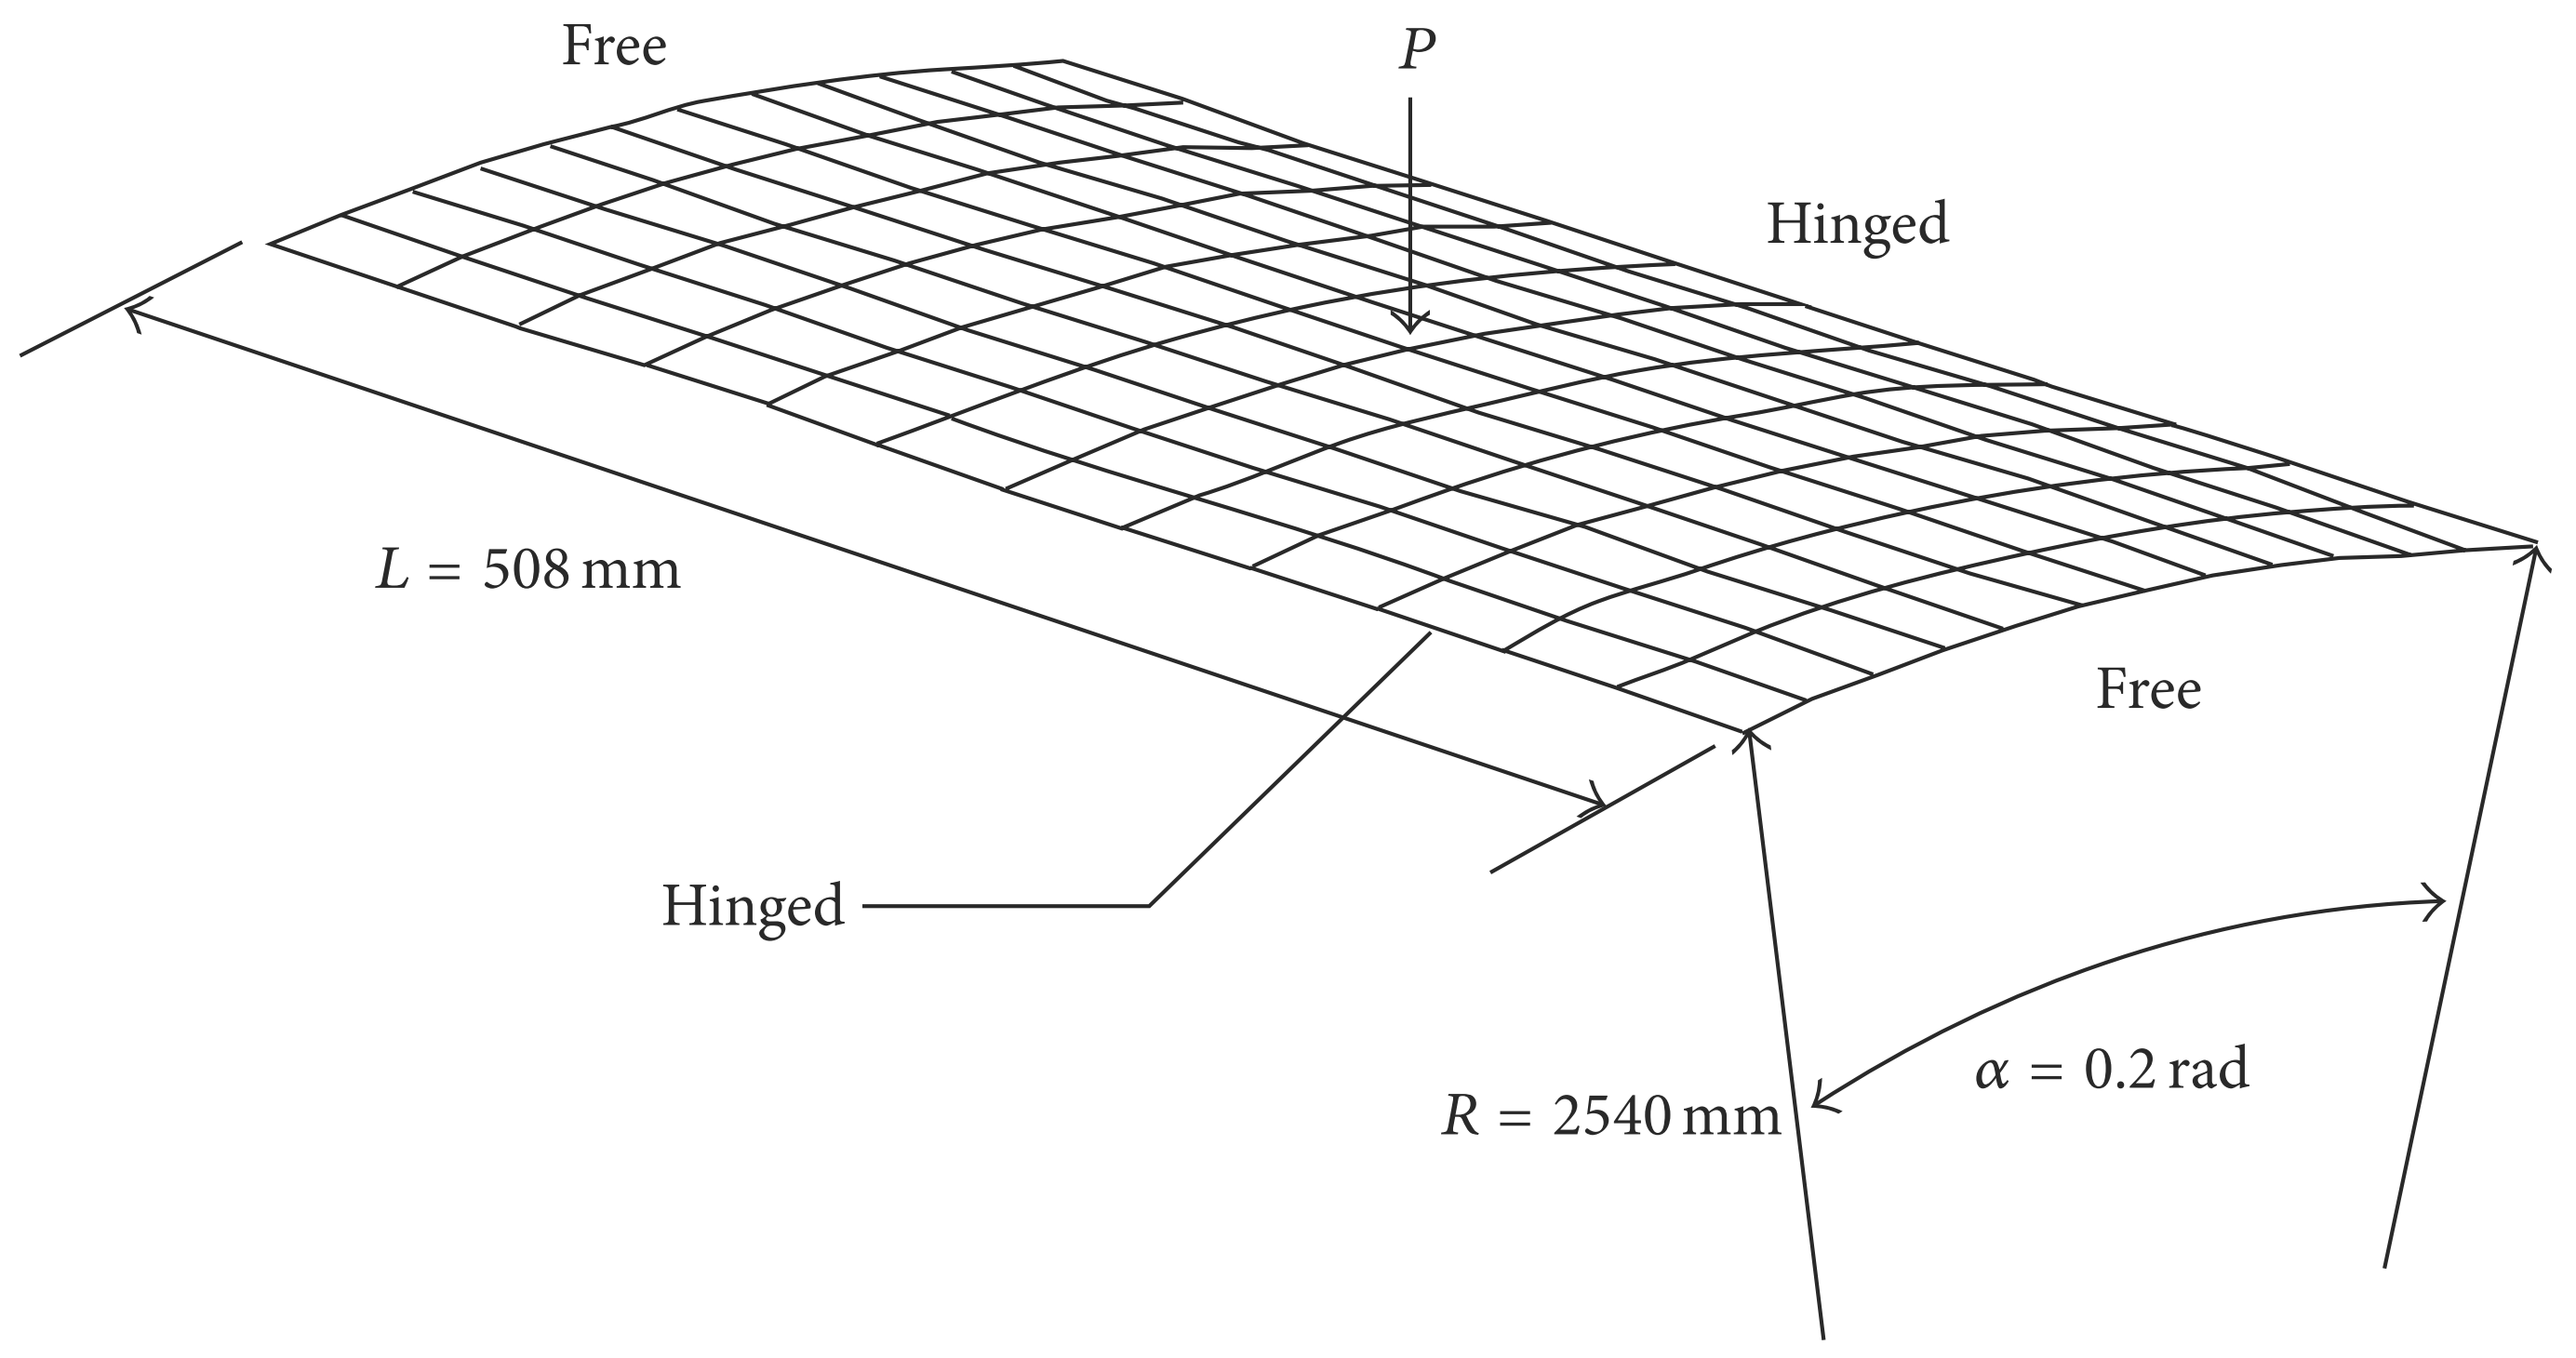
\includegraphics[width=7.3cm]
		{images/hinged_cylindrical_roof.png}}
	\subfloat[Load-displacement curve of hinged cylindrical roof]
	{\label{ref_label2}
		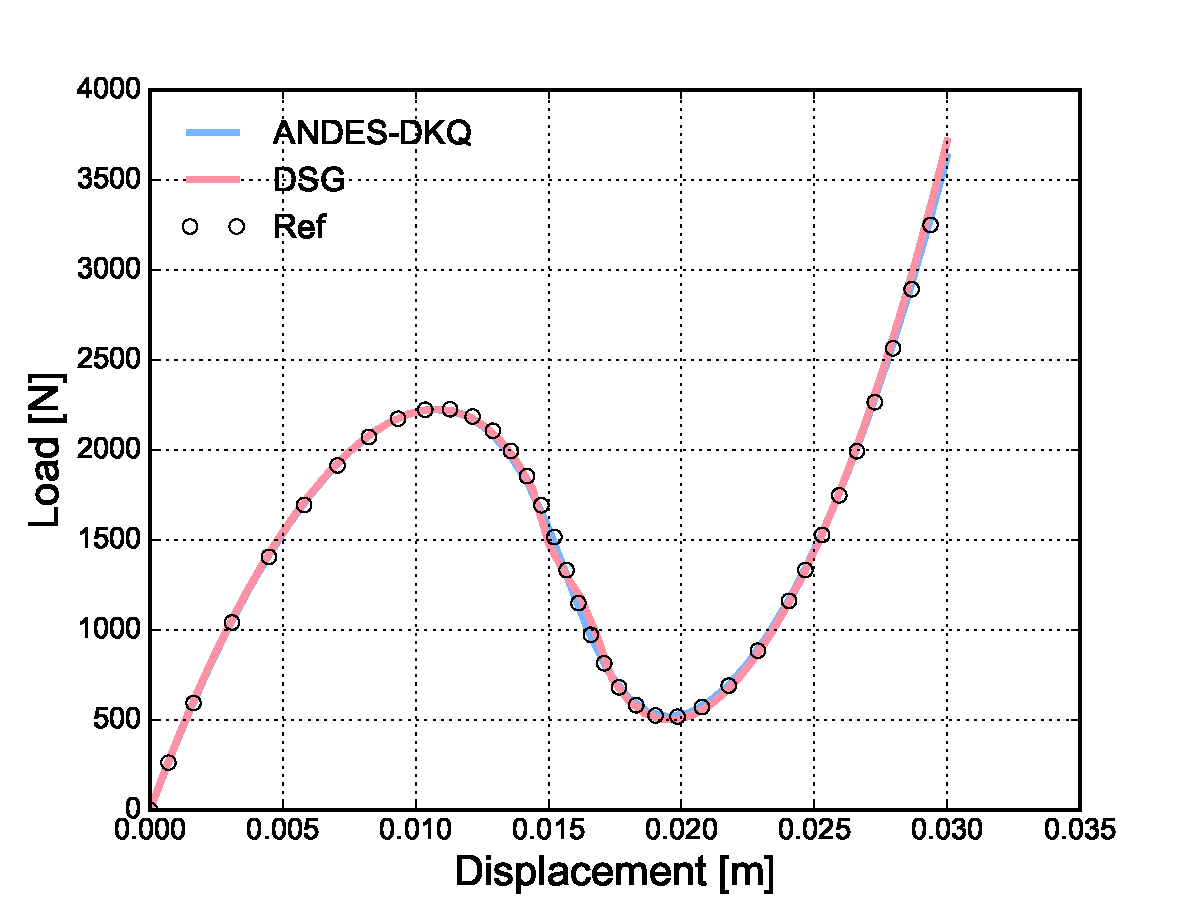
\includegraphics[width=7.3cm]
		{Load_displacement_curve_hinged_cylindrical_roof.pdf}}
	\caption{\label{ref_label_overall}Hinged cylindrical roof benchmark}
\end{figure}

\doublespacing

reference solution from \cite{Sze2004}

\subsection{Open cylinder pullout}

pullout problem

\singlespacing
\begin{figure}[H]
	%\centering
	\subfloat[Open cylinder pullout definition \cite{Sze2004}]
	{\label{ref_label1}
		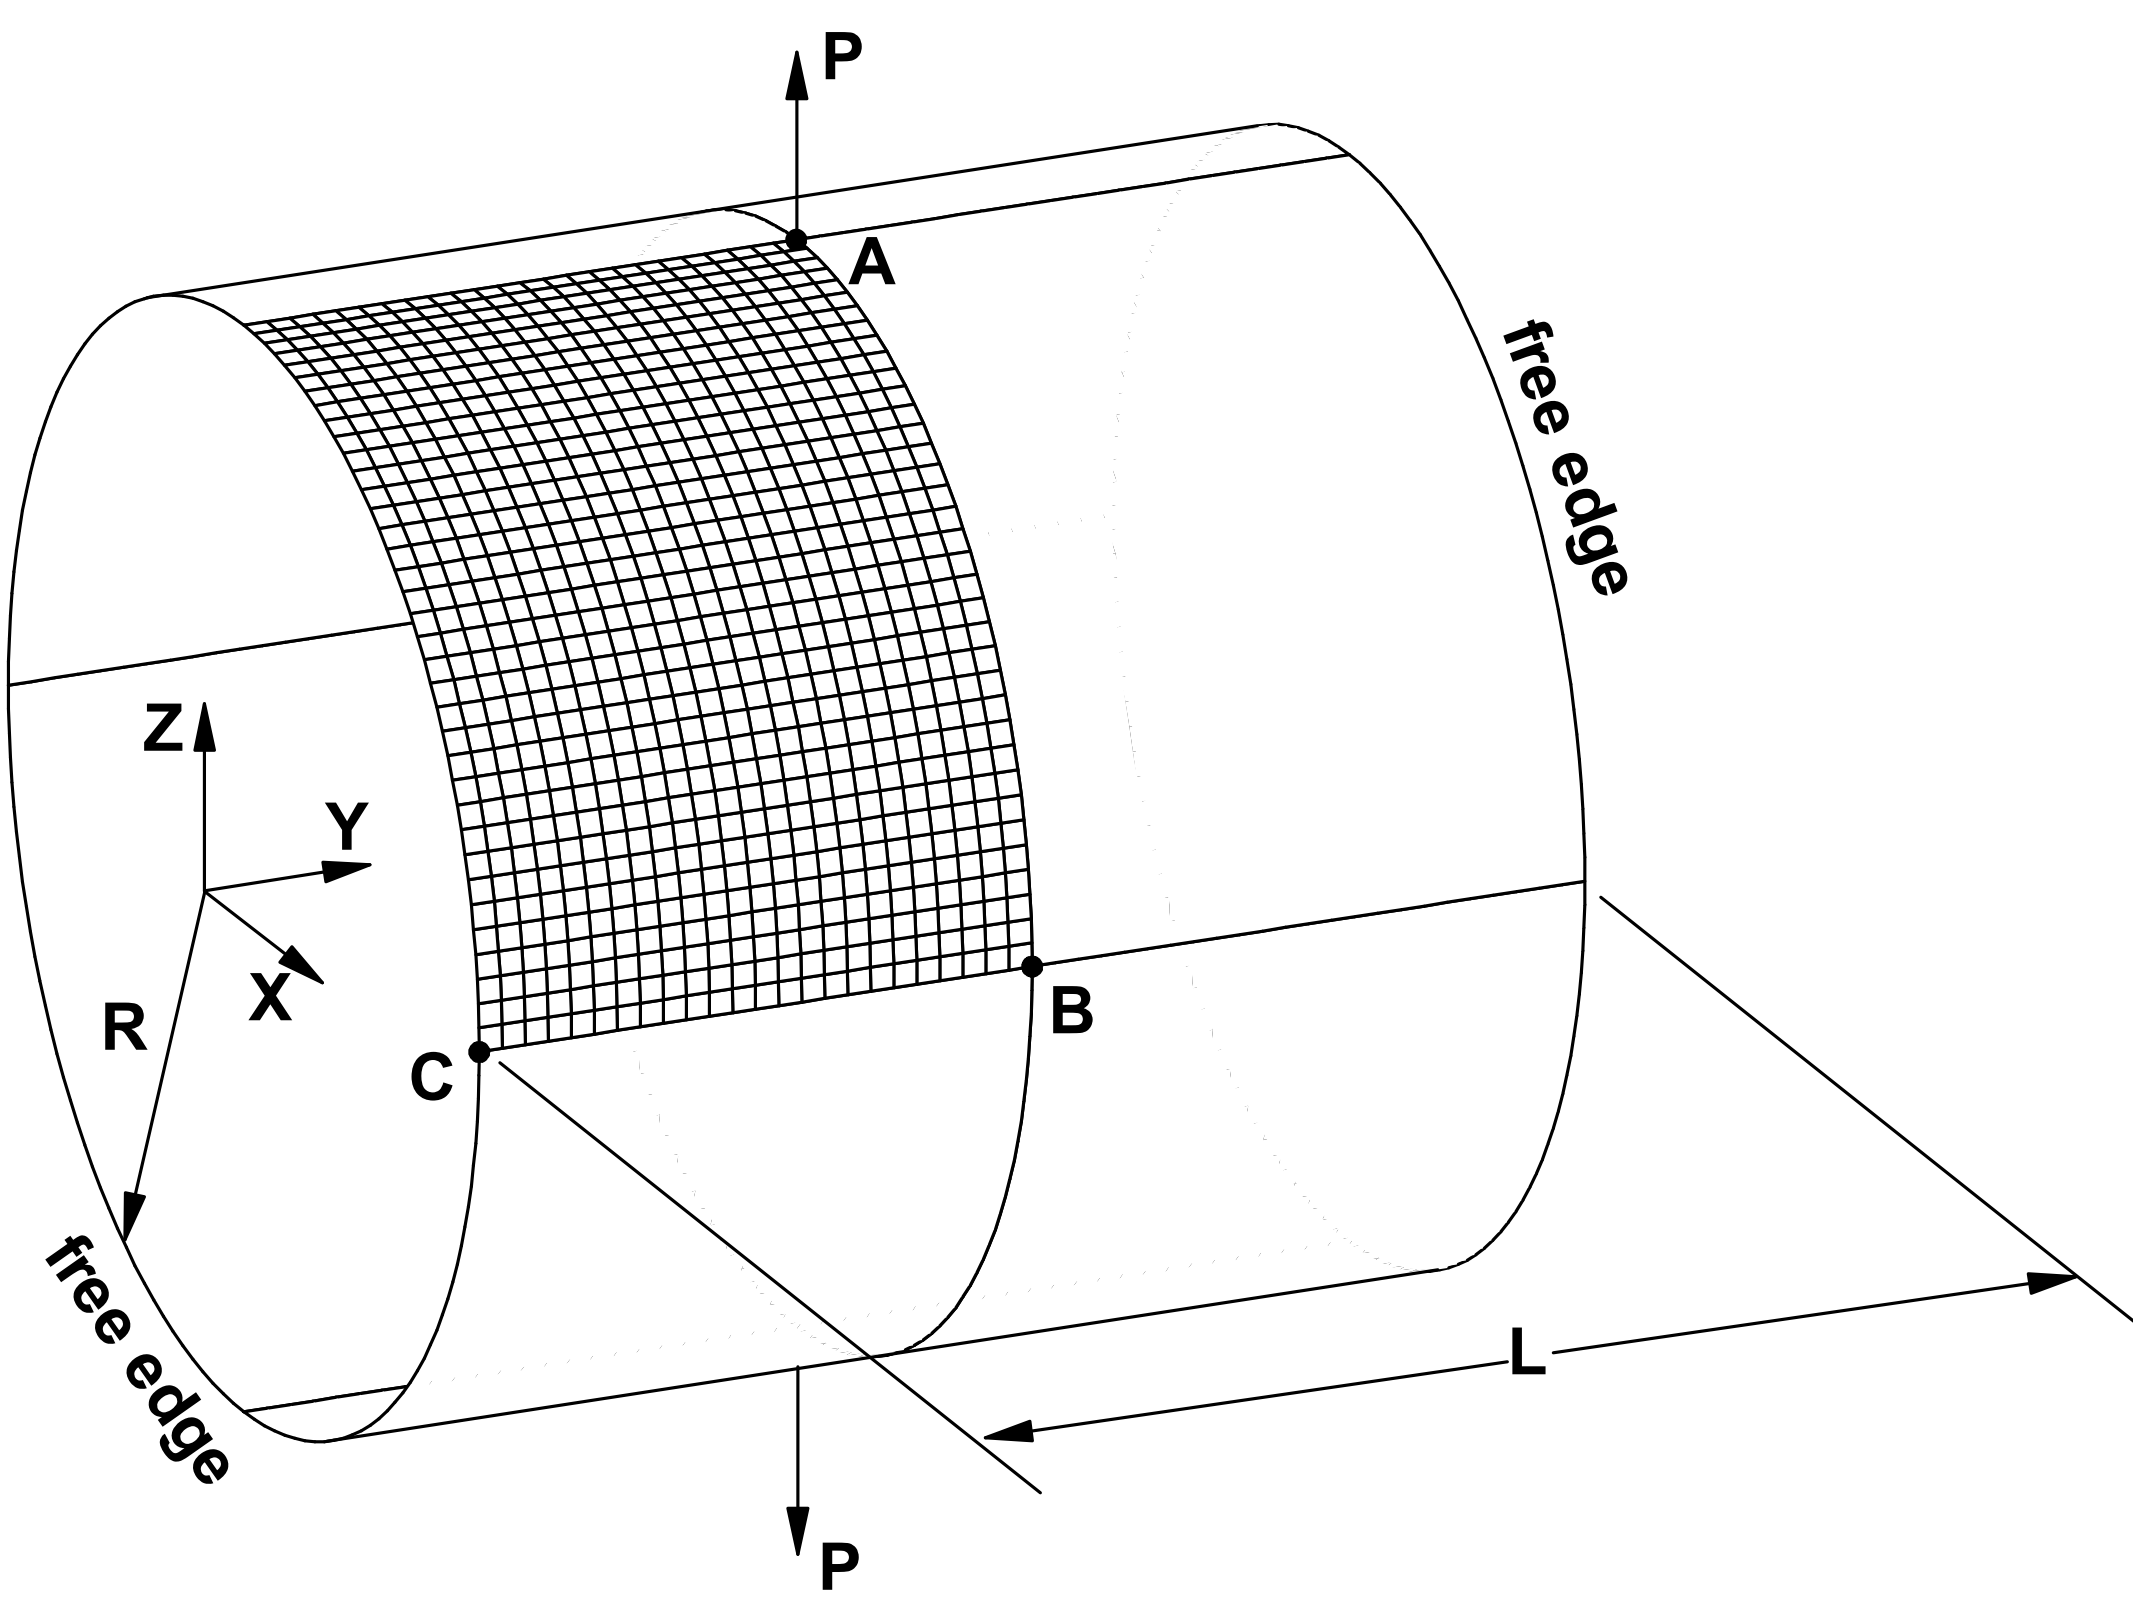
\includegraphics[width=7.3cm]
		{images/opencylinderpullout.png}}
	\subfloat[Load-displacement curve of open cylinder pullout]
	{\label{ref_label2}
		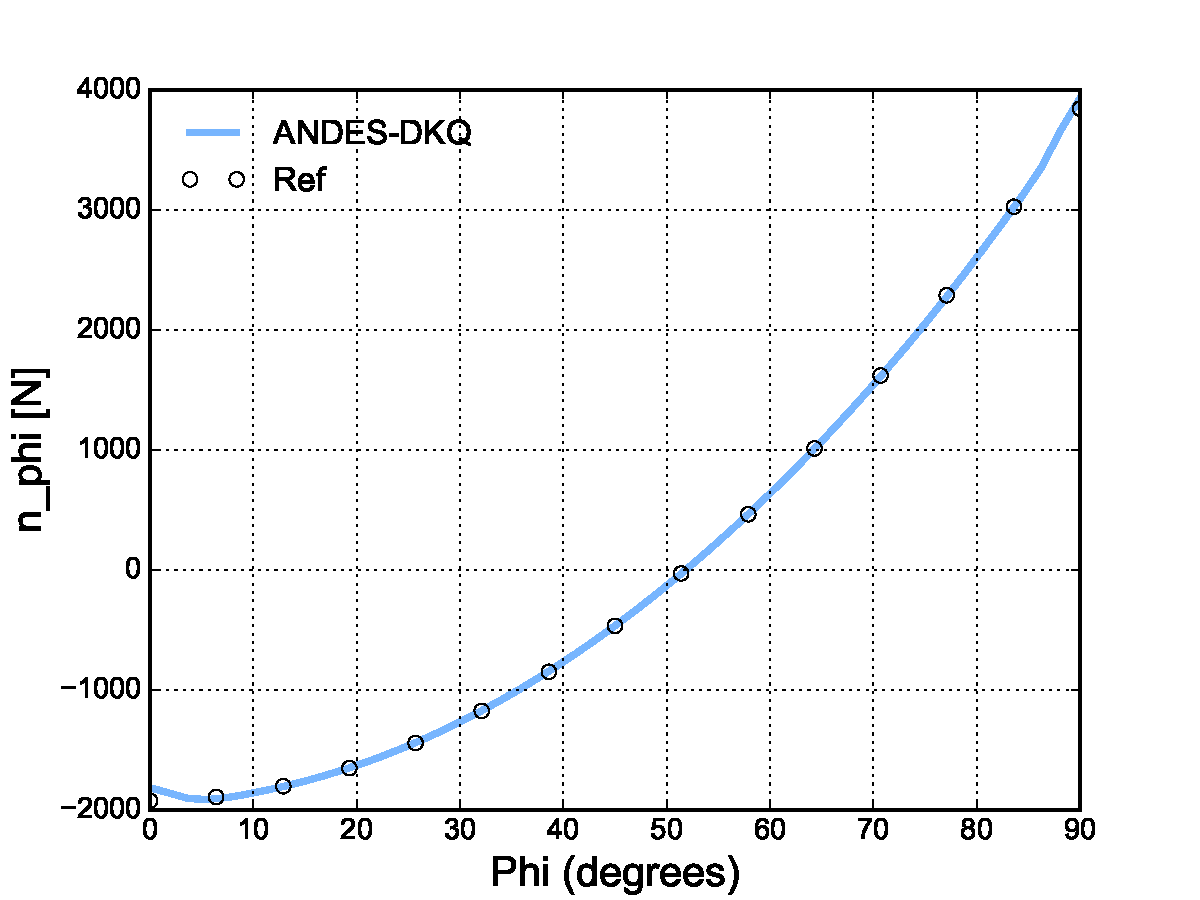
\includegraphics[width=7.3cm]
		{Load_displacement_curve_open_cylinder_pullout.pdf}}
	\caption{\label{ref_label_overall}Open cylinder pullout benchmark}
\end{figure}

\doublespacing

asdfasdf

\section{Dynamics benchmarks}

asdfasdf

\subsection{Shell pendulum}

asdfasdf

\singlespacing
\begin{figure}[H]
	%\centering
	\subfloat[Shell pendulum definition]
	{\label{ref_label1}
		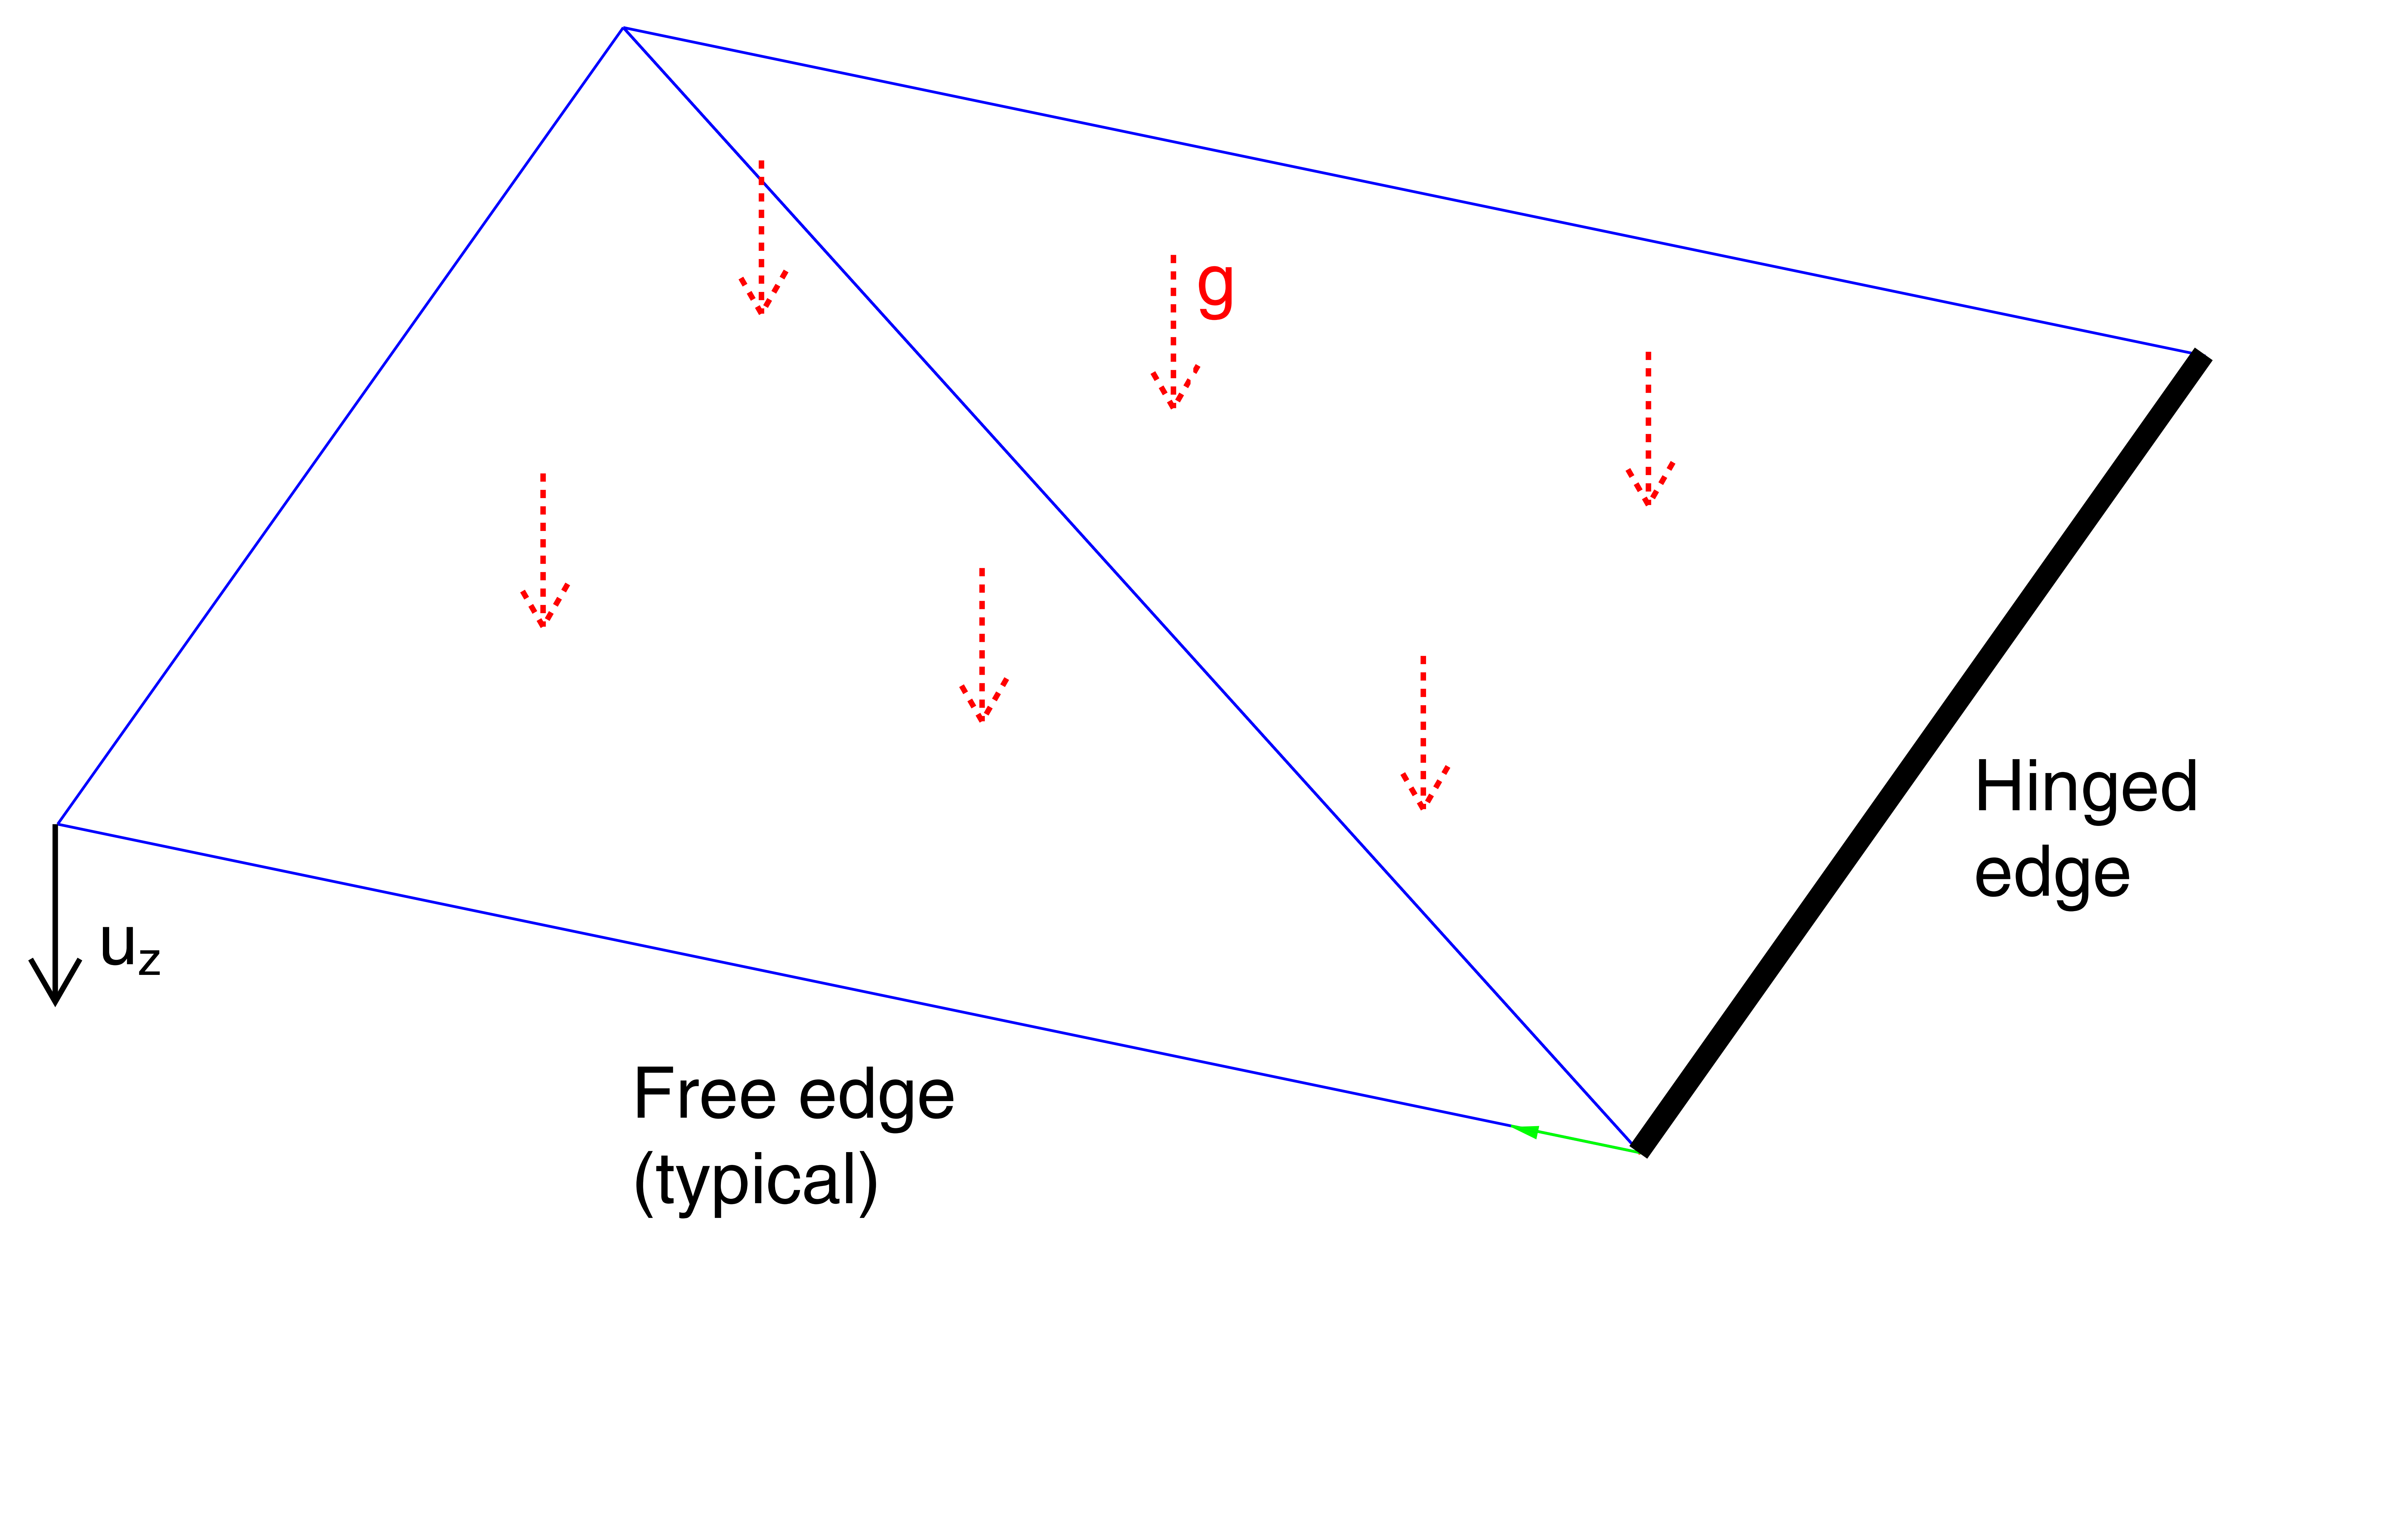
\includegraphics[width=7.3cm]
		{images/swinging_plate_problem.png}}
	\subfloat[Vertical displacement over time for shell pendulum benchmark]
	{\label{ref_label2}
		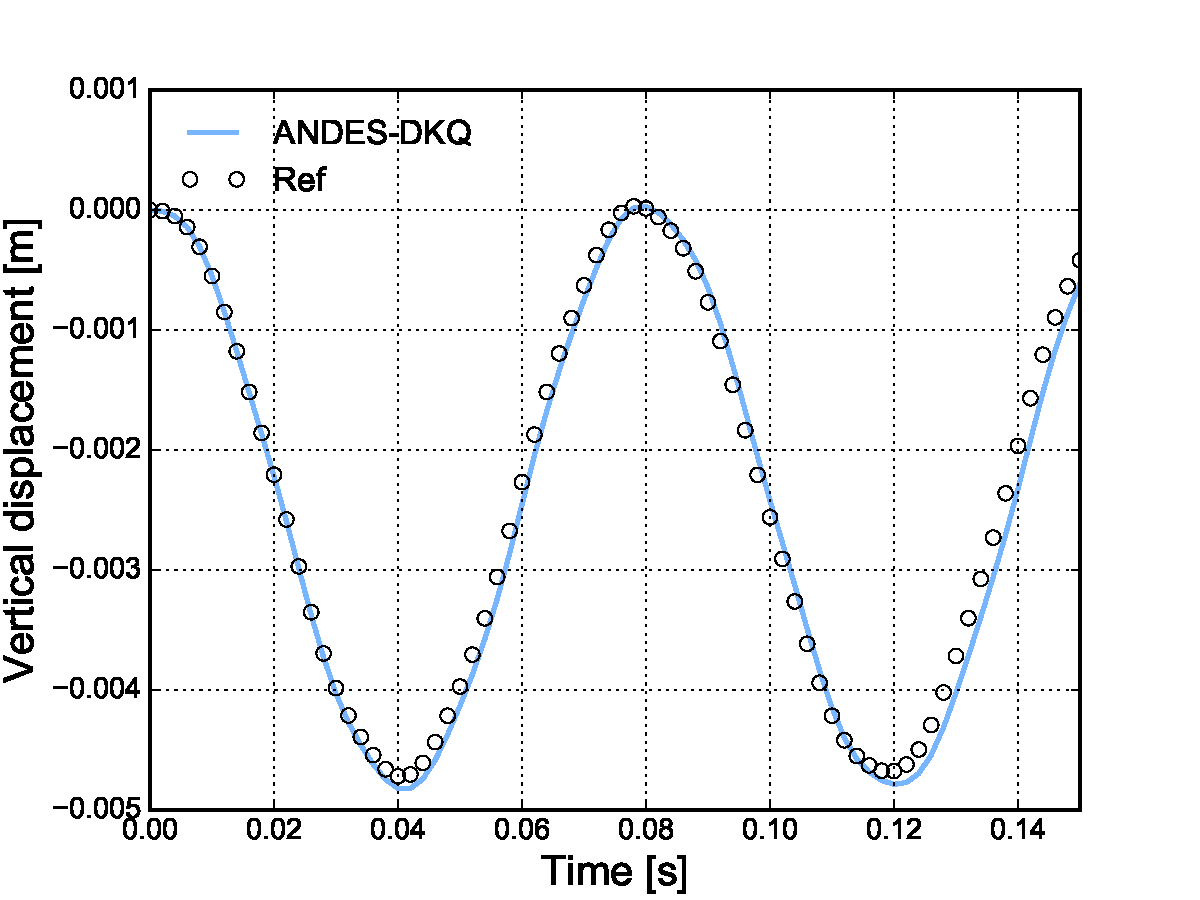
\includegraphics[width=7.3cm]
		{swinging_plate_graph.pdf}}
	\caption{\label{ref_label_overall}Shell pendulum benchmark}
\end{figure}

\doublespacing

ref is existing kratos quad

asfsdf

\subsection{Oscillating clamped plate}

adfdas


\singlespacing
\begin{figure}[H]
	%\centering
	\subfloat[Oscillating clamped plate definition]
	{\label{ref_label1}
		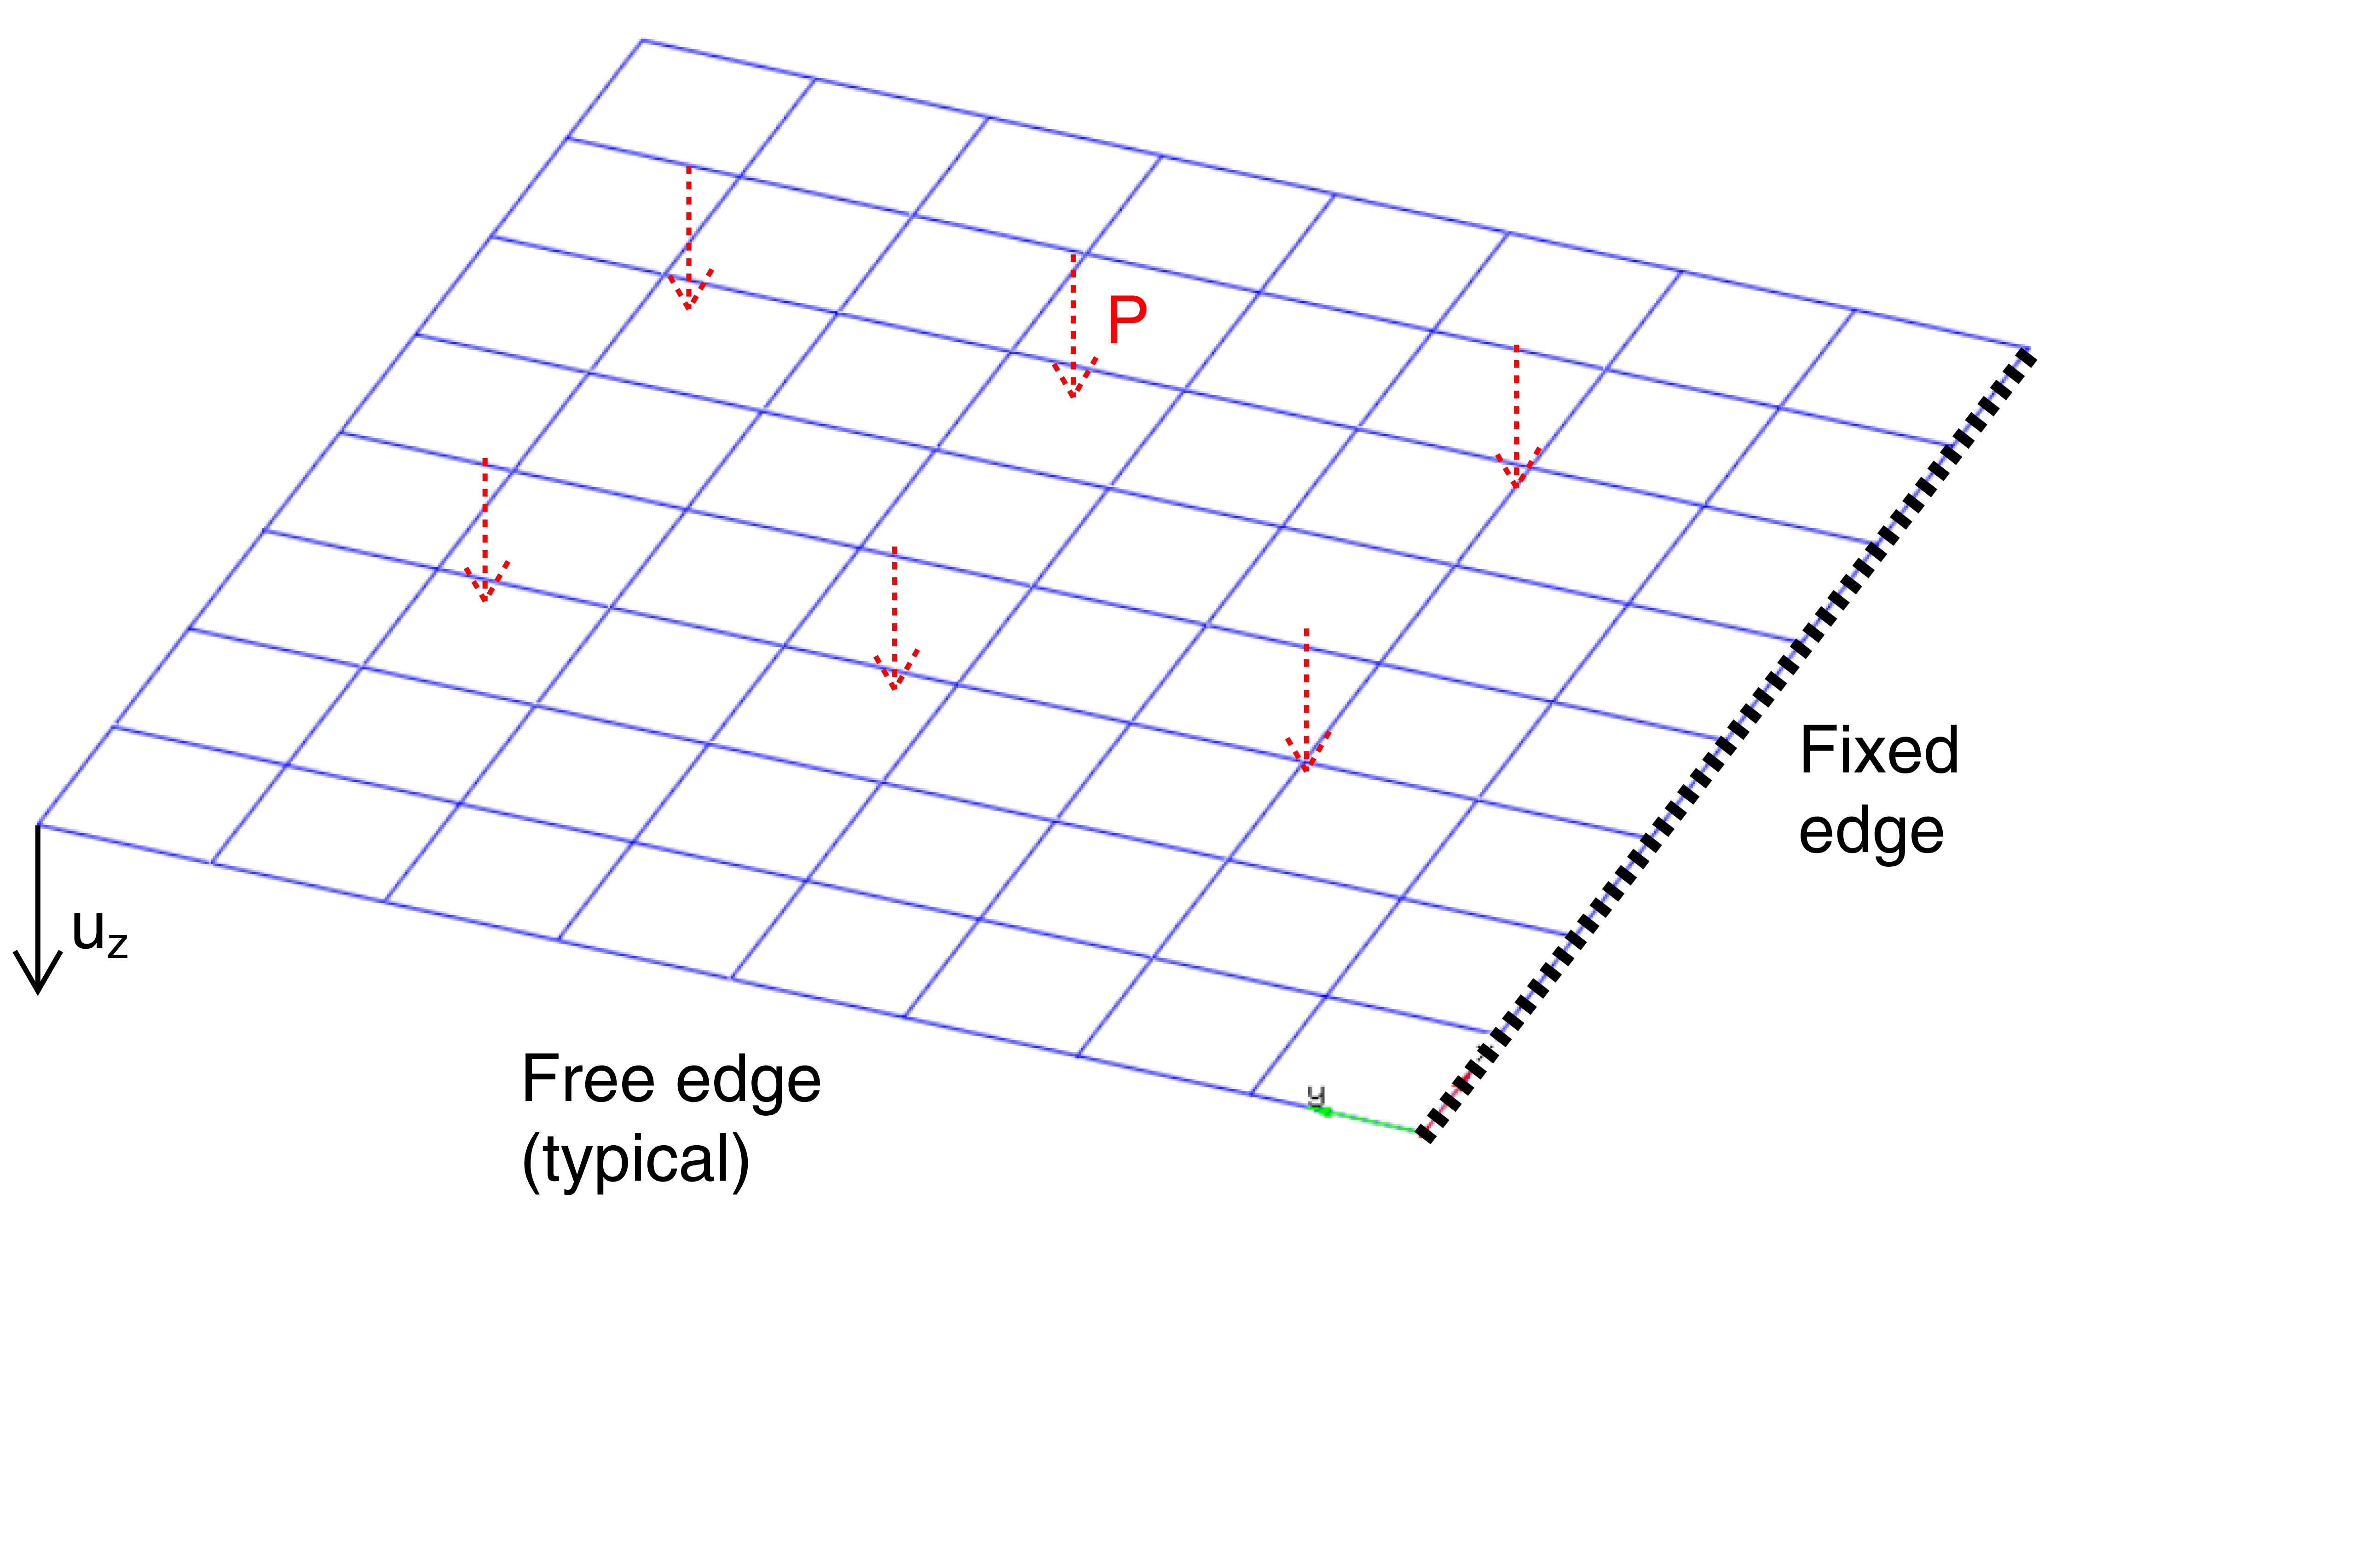
\includegraphics[width=7.3cm]
		{images/quad_bend_problem.png}}
	\subfloat[Vertical displacement over time for Oscillating clamped plate benchmark]
	{\label{ref_label2}
		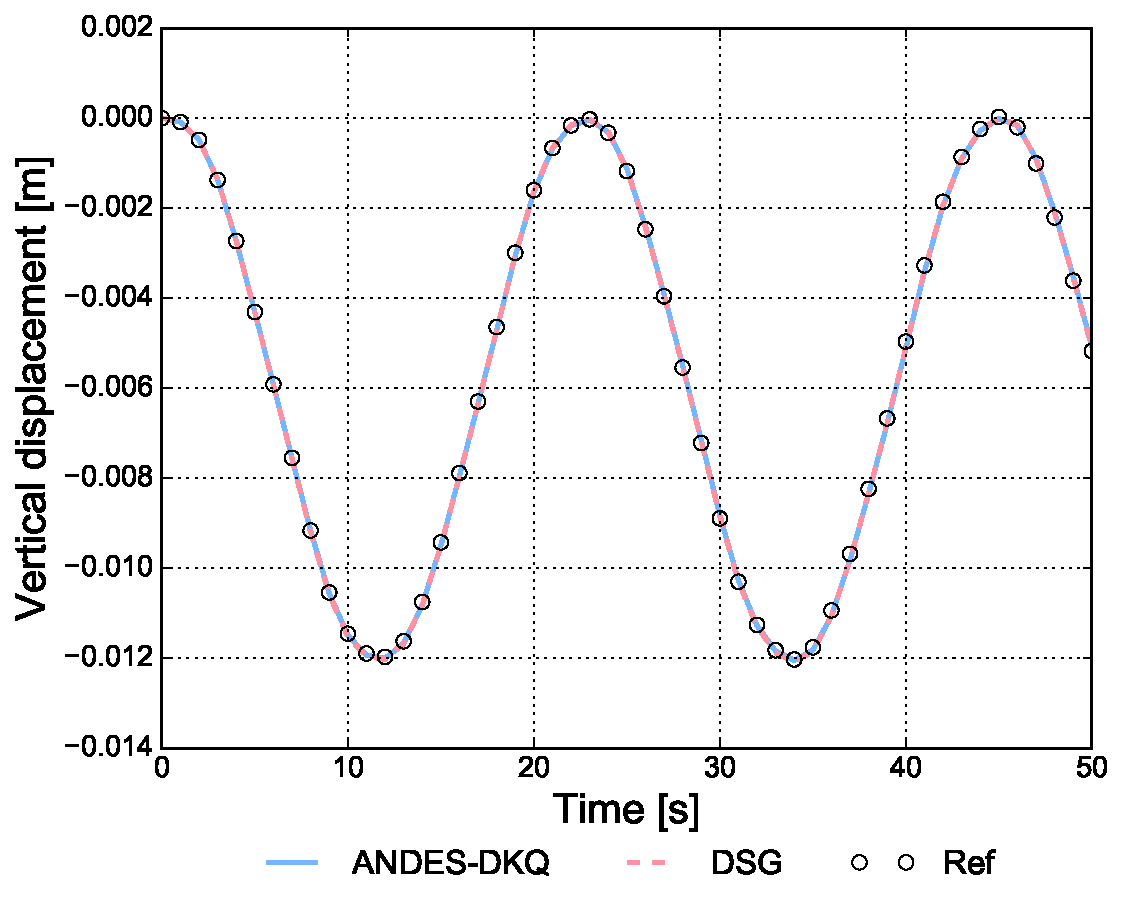
\includegraphics[width=7.3cm]
		{quad_bend_graph.pdf}}
	\caption{\label{ref_label_overall}Oscillating clamped plate benchmark}
\end{figure}

\doublespacing

ref is existing kratos quad



